Les courbes et surfaces de Bézier ont été implémentées au moyen de 2 classes en C++. L'implémentation fait s'appuyer les surfaces de Bézier sur un ensemble de courbes de contrôle
qui elles même s'appuient sur un ensemble de points de contrôle.

La déformation globale de torsion agit sur tous les sommets du maillage et prend en paramètre un axe de torsion ainsi qu'une "intensité" de torsion exprimée en "degrés par unité" dans
les figures ci-dessous. Les 3 déformations locales (translations) appliquées à la surface de Bézier agissent sur tous les sommets du maillage mais l'intensité de la déformation
est modulée par une fonction à support compact de type smoothstep ($x^2(3 -2x)$) qui prend en argument la distance au centre de la déformation. Le centre de la déformation
est précisé par un des sommets du maillage dans cette implémentation.

\begin{figure}[h!]
	\adjustbox{center}{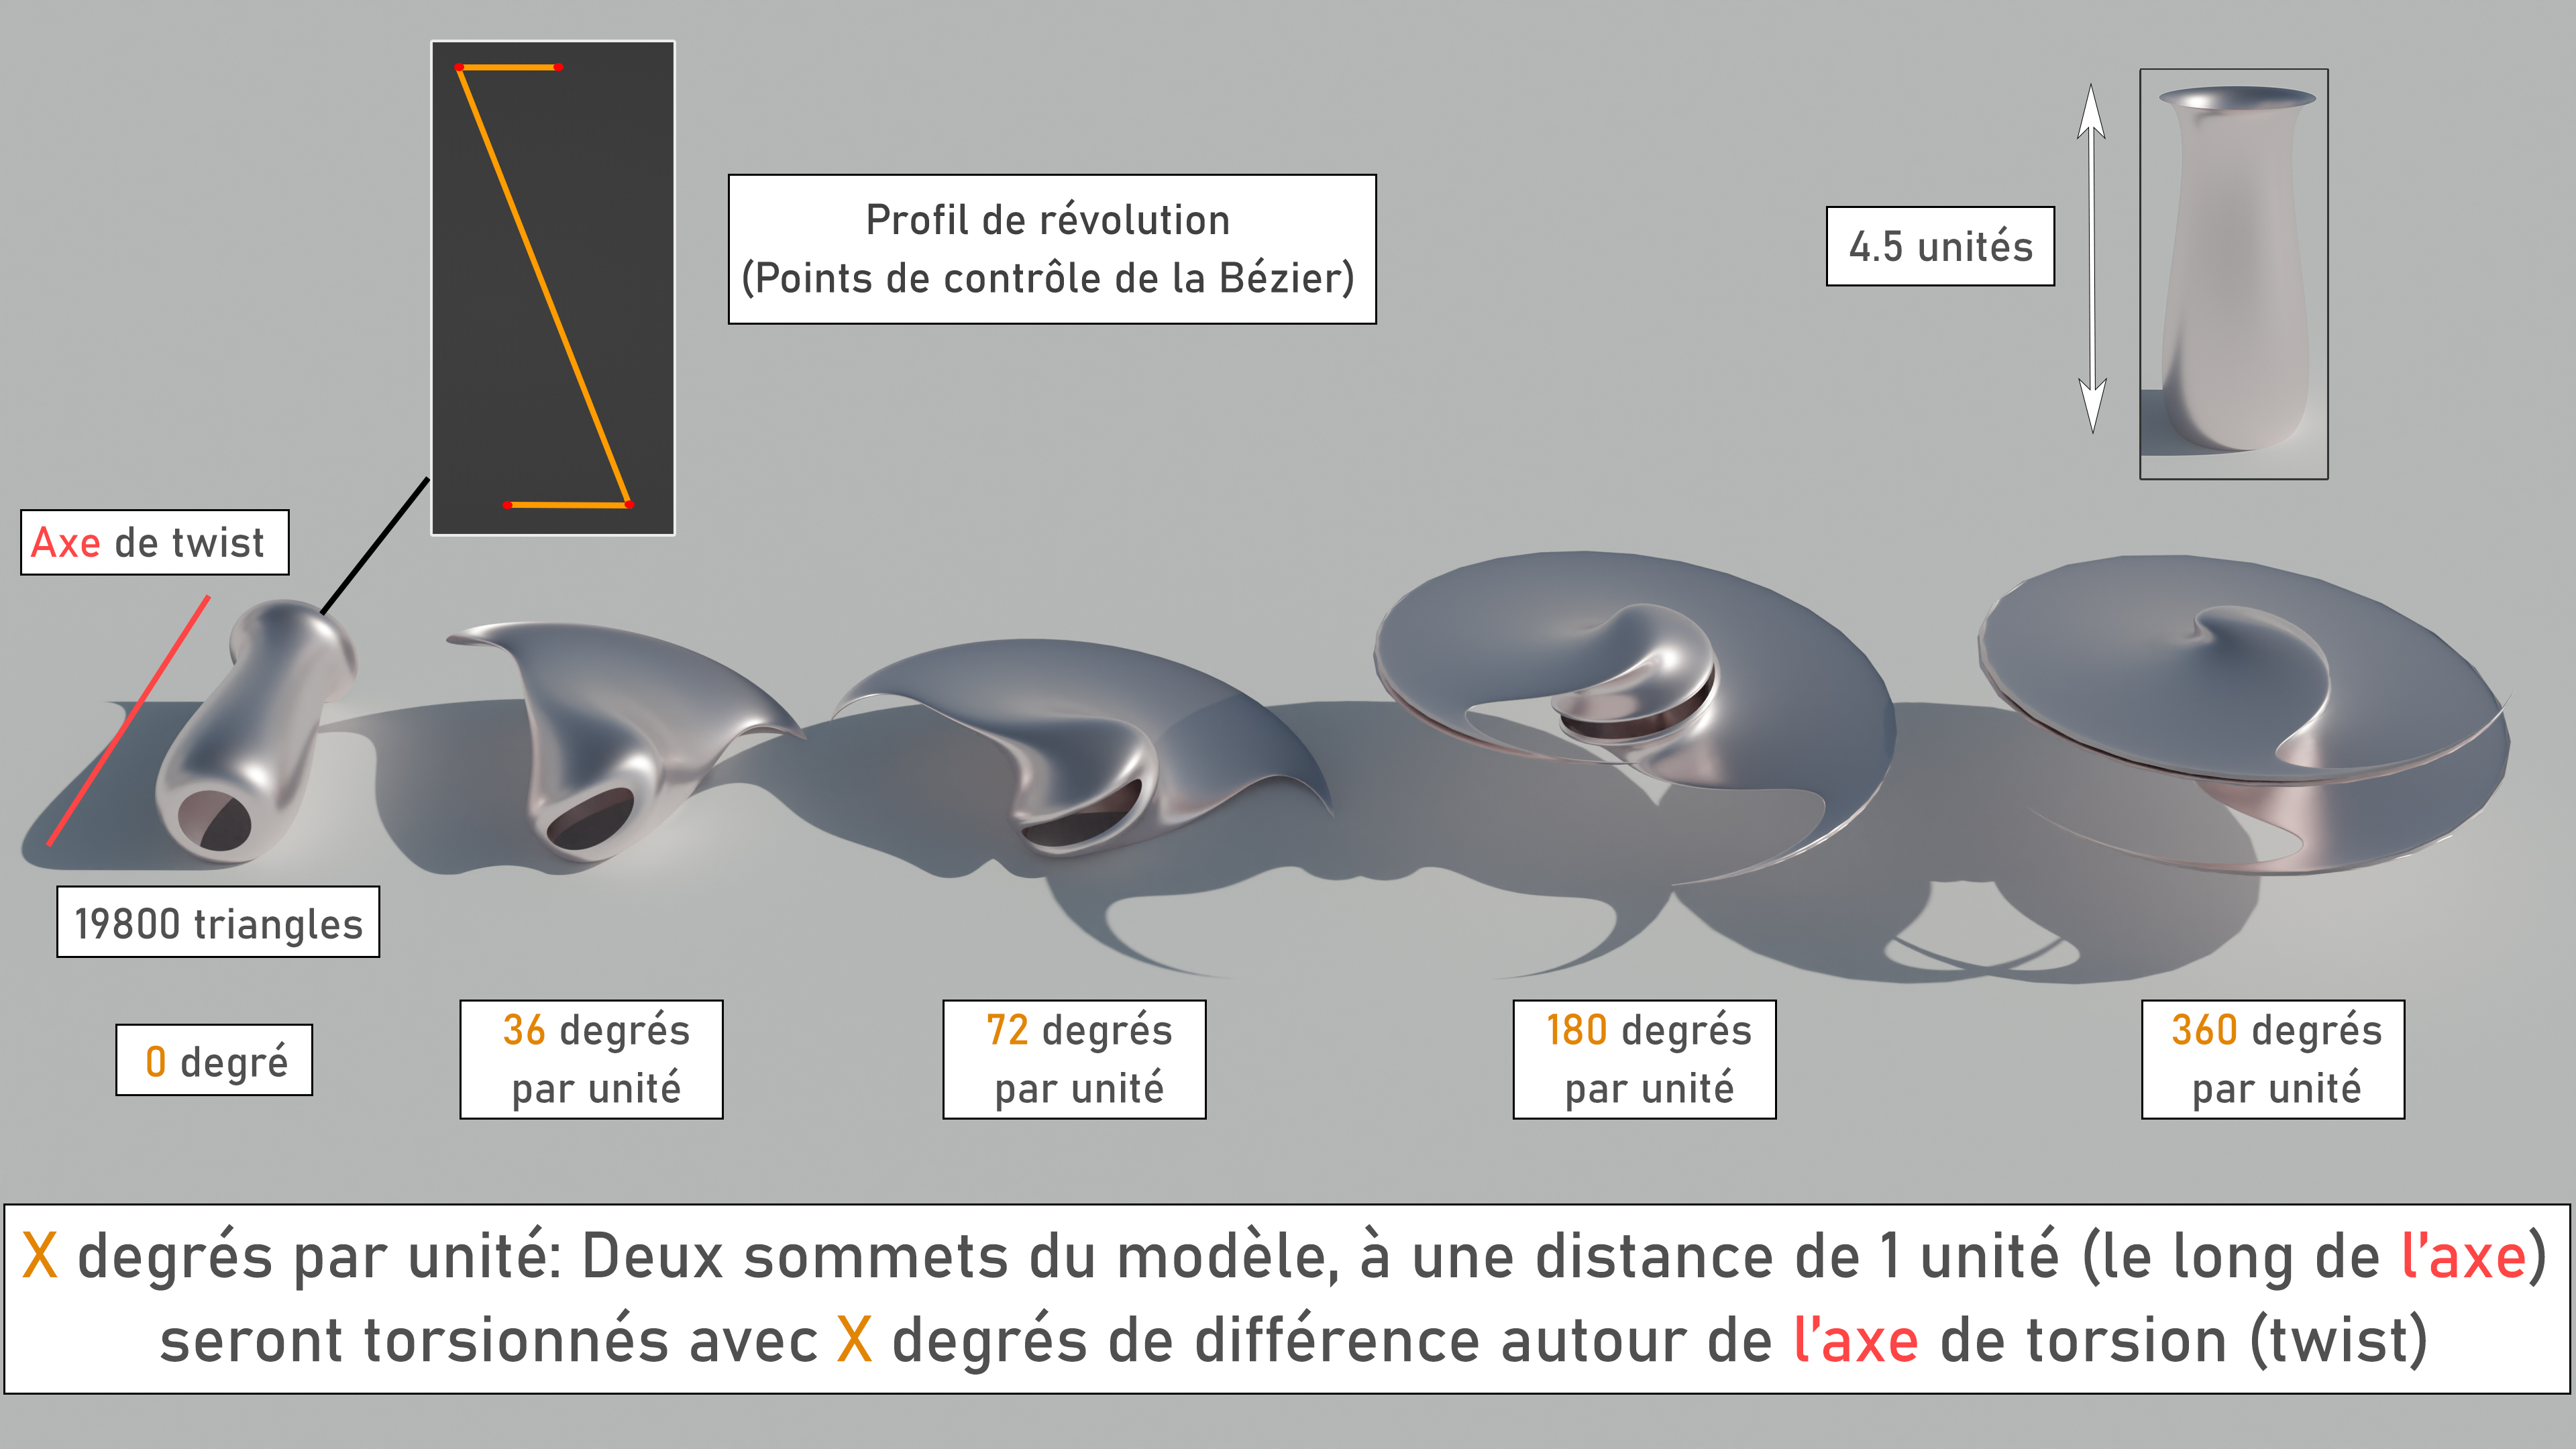
\includegraphics[width=1\textwidth]{Captures/Revolution.jpg}}

	\caption{Rendu Blender d'une surface de révolution modélisée, maillée et déformée globalement (torsion/twist) avec TinyMesh}
	\label{ref}
\end{figure}
\FloatBarrier

\begin{figure}[h!]
	\adjustbox{center}{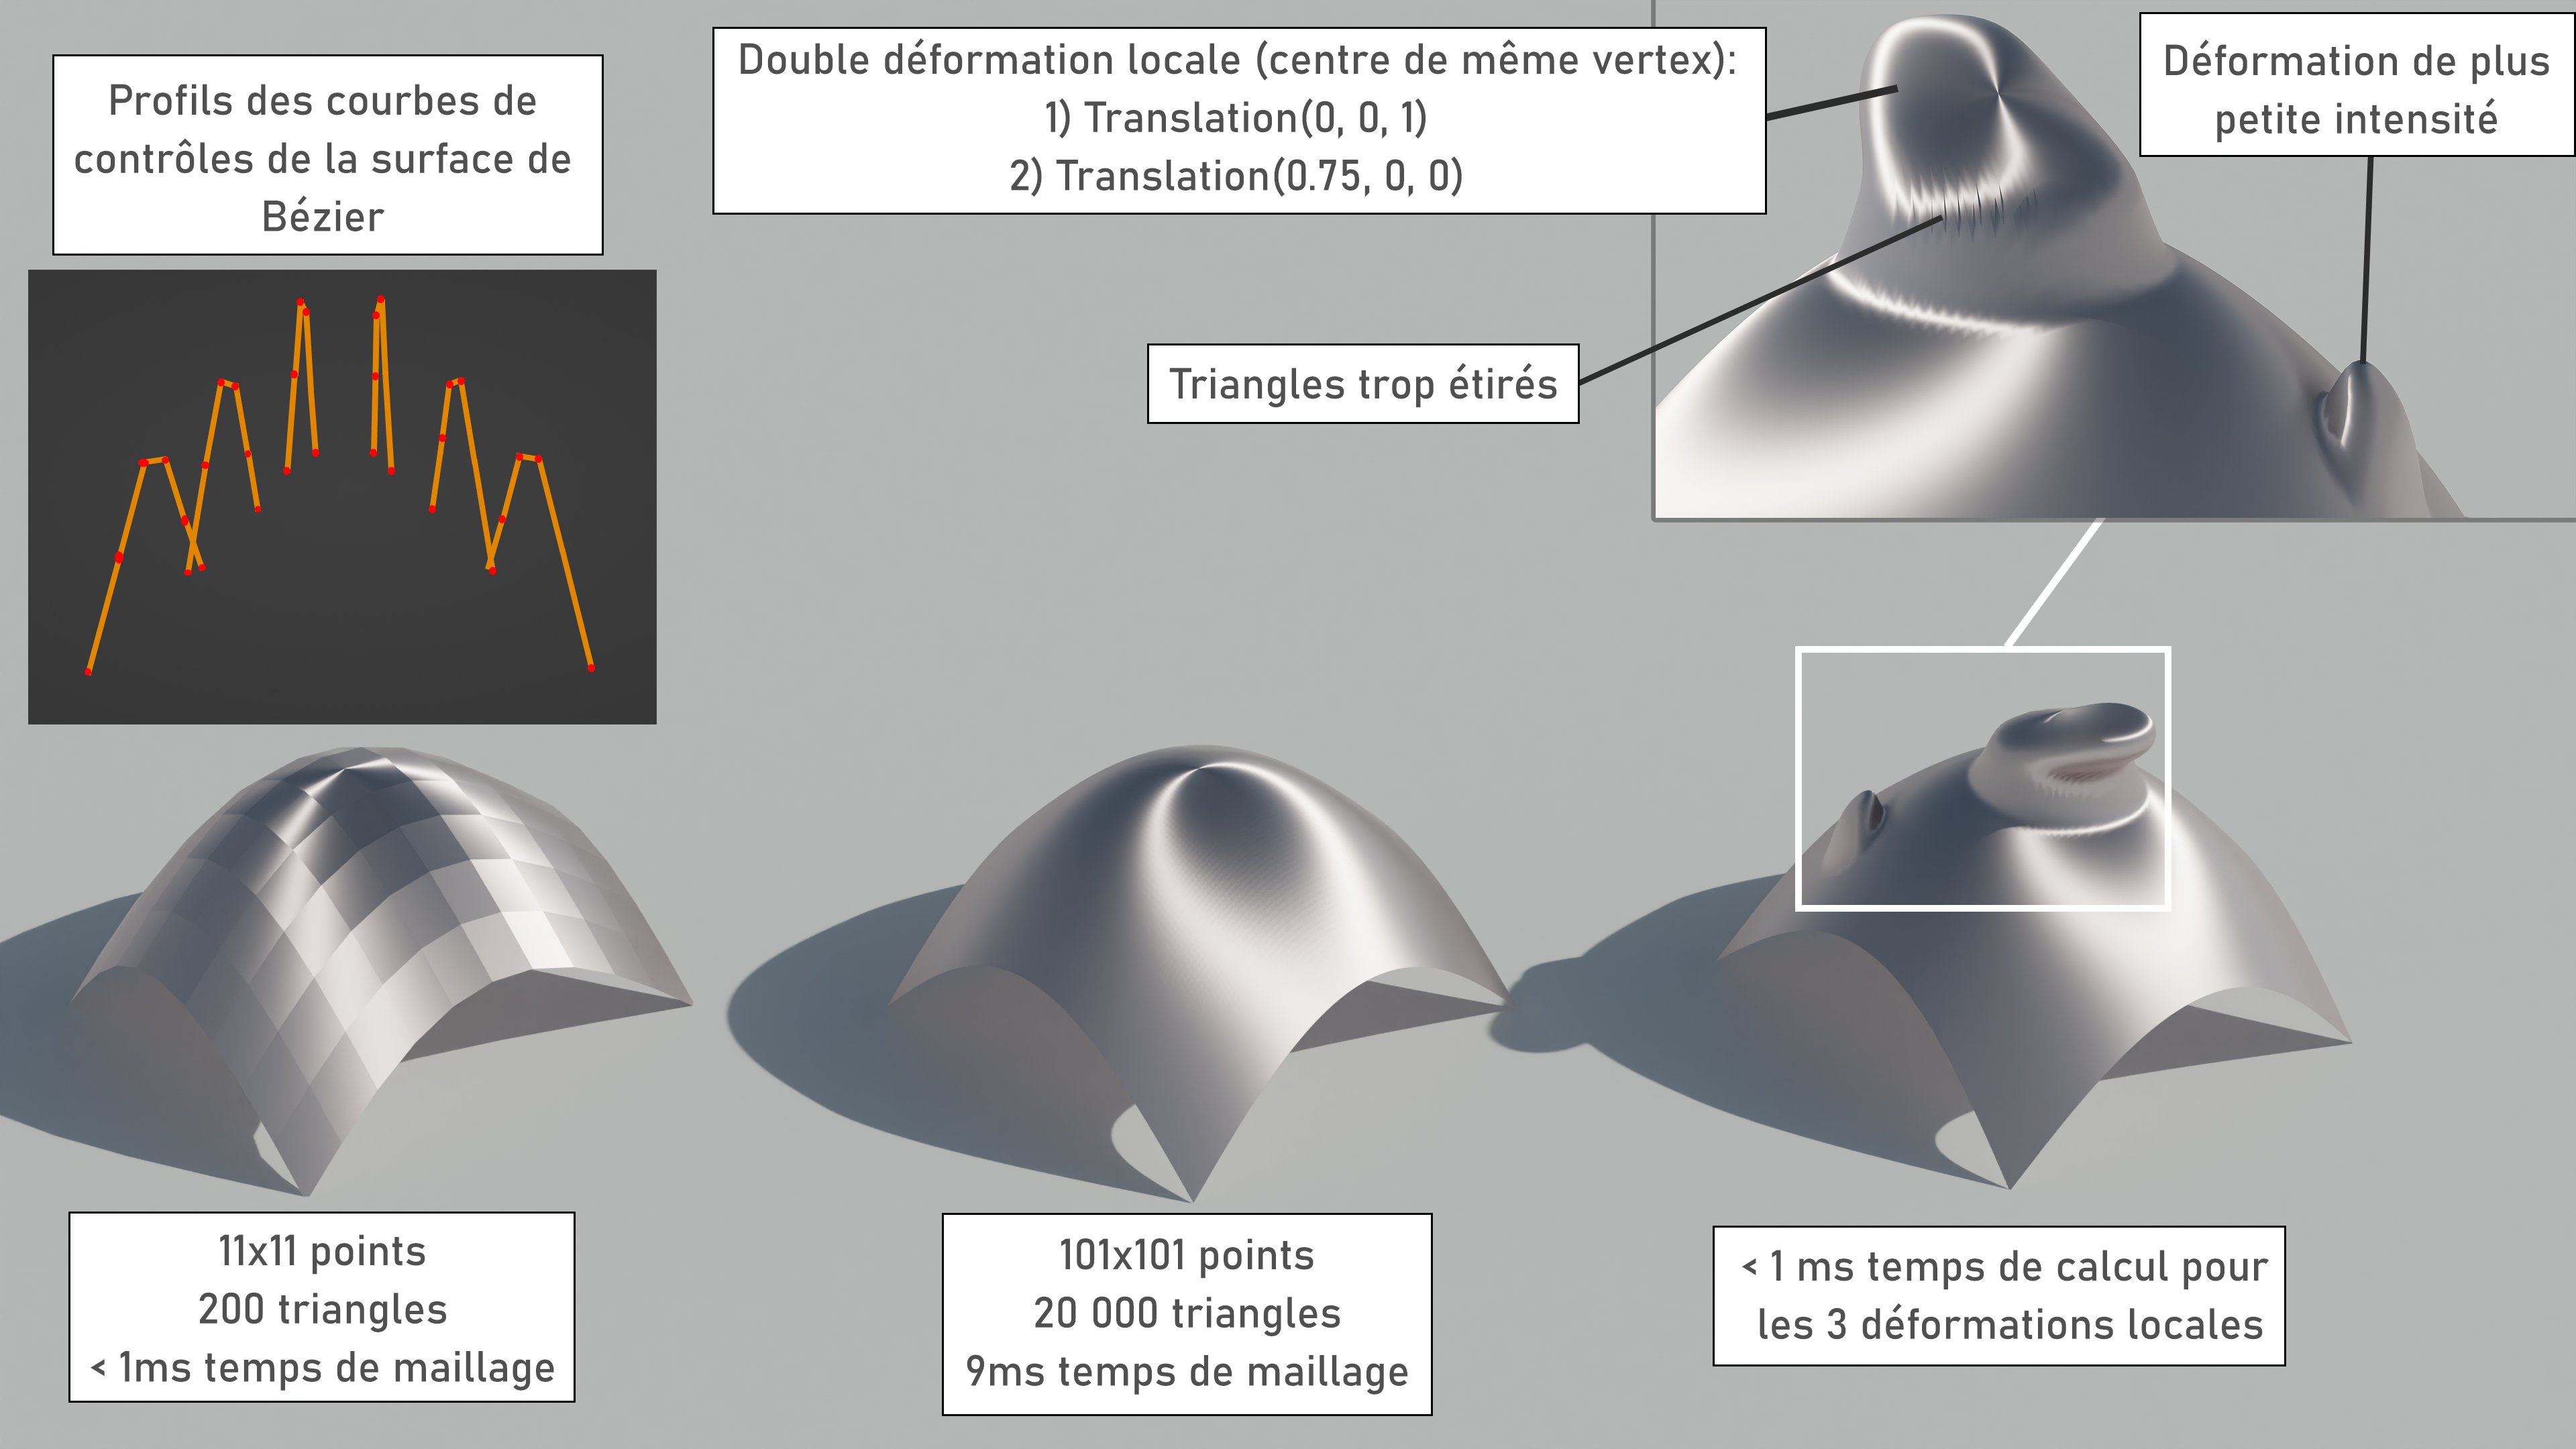
\includegraphics[width=1\textwidth]{Captures/Bezier.jpg}}

	\caption{Rendu Blender d'une surface de Bézier à différentes résolutions de maillage modélisée, maillée et déformée localement (translation atténuée) avec TinyMesh}
	\label{ref}
\end{figure}
\FloatBarrier

.

